%\documentclass[a4paper,12pt,BCOR12mm,toc=bibliography]{scrbook}
\documentclass[a4paper,11pt,BCOR11mm,toc=bibliography]{scrbook} % mod 12 pt BCOR11mm
\usepackage{amsmath}
\usepackage{amssymb}
\usepackage{graphicx}
\usepackage{dsfont}
\usepackage[makeroom]{cancel} % for crossing out terms in Eqs.

\usepackage{geometry}
\geometry{a4paper,top=3.2cm,bottom=4.8cm,left=3.1cm,right=3.1cm,heightrounded,bindingoffset=0mm}


\usepackage{hyperref}
\hypersetup{
  colorlinks   = true, 
  urlcolor     = black, 
  linkcolor    = black,
  citecolor   = black 
}

\graphicspath{{../pics/}}           %set subdirectory for figures
\usepackage{floatrow}   % for side figures that can be shifted

\usepackage{booktabs}  %for nice tables
\usepackage{textcomp}  %for upright \mu in units, use \textmu
\usepackage{wrapfig}   %for wrapped figures

\usepackage[english]{babel}  %language specific support
\usepackage{cite}                   %e.g. multiple citations appear as [1-5] instead of [1,2,3,4,5]

%headings /footnote controls:
%    \usepackage[automark]{scrpage2}
%    \pagestyle{scrheadings} \clearscrheadfoot
%    %\renewcommand*\chaptermarkformat{}  %switch off chapter numbering in headline
%    %\renewcommand*\sectionmarkformat{}  %switch off section numbering in headline
%    \lehead{\pagemark\quad\headmark}
%    \rohead{\headmark\quad\pagemark}
%    %\ohead{\pagemark}       % page numbering on headline, outside
%    %\chead{\headmark}       % chapter/section title on headline, centered
%
%    \renewcommand{\headfont}{\sffamily\slshape}  %font of chapter/section title
%    \renewcommand{\pnumfont}{\sffamily\bfseries} %font of page number
%    \setheadsepline[text]{.4pt}   % line under the headings


%figure captions:
    \addtokomafont{captionlabel}{\sffamily\bfseries}  %bold figure labels
    \setcapindent{2em}                              %figure caption indents
    \usepackage{sidecap}  %allow for captions left from the figure \begin{SCfigure}...

%margin changes:
    \addtolength{\topmargin}{1.5em}  %shift everything down by X
%    \setlength{\oddsidemargin}{5mm} 
%    \setlength{\evensidemargin}{5mm}

%\usepackage[numbers,square]{natbib}

%BIBLATEX:
    %\usepackage[style=science,article-title,maxnames=1000]{biblatex}
    %\renewcommand{\mkbibbrackets}[1]{[#1]}
    %\addbibresource{eit} \addbibresource{phdthesis_misc}
    %\addbibresource{D:/Lab_Software/literature/paper_others}
    
% general
\newcommand{\tol}[3]{\hbox{\rule{0pt}{15pt}${#1}^{+{#2}}_{-{#3}}$}} % assymetric error bars
\newcommand{\f}[2]{#1 [#2]}  %function defintition with [], forced in by Anna :D
\newcommand{\F}[2]{#1 \left[#2\right]}
\newcommand{\dx}{\,\mathrm{d}x} % for integral
\newcommand{\abs}[1]{\left| #1 \right|} % for absolute value
\newcommand{\avg}[1]{\overline{#1}} % for average
\newcommand{\real}[0]{\ensuremath{\text{Re}}} % real part
\newcommand{\imag}[0]{\ensuremath{\text{Im}}} % imaginary part

% color boxes for marking to dos
\usepackage{color}
\newcommand{\cbox}[1]{\colorbox{yellow}{#1}}   % roter Text in gelber Box
% encircled numbers
\usepackage{tikz}
\definecolor{Myblue}{cmyk}{0.71,0.53,0,0.12}
\newcommand{\kreis}[1]{{\tiny \textcolor{Myblue}{\tikz \node[draw,circle]{#1};}}}
\newcommand{\pos}[1]{{\textcolor{Myblue}{Pos.~#1}}}

%QUANTUM
\newcommand{\ket}[1]{|{#1}\rangle}
\newcommand{\bra}[1]{\langle{#1}|}
\newcommand{\prj}[1]{\ket{#1}\bra{#1}}
\newcommand{\ketbra}[2]{\ket{#1}\bra{#2}}
\newcommand{\expect}[1]{\left< #1 \right>} % for expectaiotn value
\newcommand{\Tr}[1]{{\rm Tr} \left[#1 \right]} % trace
\newcommand{\ua}[0]{{\ket{\uparrow}}} % spin up
\newcommand{\da}[0]{{\ket{\downarrow}}} % spin down

% units
\usepackage{xspace}

\newcommand{\amu}{\,\ensuremath{\text{u}}\xspace}

\newcommand{\muK}{\,\ensuremath{\mu\text{K}}\xspace}
\newcommand{\mK}{\,\ensuremath{\text{mK}}\xspace}

\newcommand{\ohm}{\,\ensuremath{\Omega}\xspace} % \xspace ensures correct spacing after command
\newcommand{\kohm}{\,\ensuremath{\text{k}\Omega}\xspace}
\newcommand{\Mohm}{\,\ensuremath{\text{M}\Omega}\xspace}

\newcommand{\rad}{\,\ensuremath{\text{rad}}\xspace}

\newcommand{\mbar}{\,\ensuremath{\text{mbar}}\xspace}

\newcommand{\ps}{\,\ensuremath{\text{ps}}\xspace}
\newcommand{\ns}{\,\ensuremath{\text{ns}}\xspace}
\newcommand{\mus}{\,\ensuremath{\mu\text{s}}\xspace}
\newcommand{\ms}{\,\ensuremath{\text{ms}}\xspace}
\newcommand{\s}{\,\ensuremath{\text{s}}\xspace}

\newcommand{\m}{\,\ensuremath{\text{m}}\xspace}
\newcommand{\cm}{\,\ensuremath{\text{cm}}\xspace}
\newcommand{\mm}{\,\ensuremath{\text{mm}}\xspace}
\newcommand{\mum}{\,\ensuremath{\mu\text{m}}\xspace}
\newcommand{\nm}{\,\ensuremath{\text{nm}}\xspace}
\newcommand{\pim}{\,\ensuremath{\text{pm}}\xspace}
\newcommand{\fm}{\,\ensuremath{\text{fm}}\xspace}

\newcommand{\G}{\,\ensuremath{\text{G}}\xspace}

\newcommand{\counts}{\,\ensuremath{\text{ms}^{-1}}\xspace}

\newcommand{\Hz}{\,\ensuremath{\text{Hz}}\xspace}
\newcommand{\kHz}{\,\ensuremath{\text{kHz}}\xspace}
\newcommand{\MHz}{\,\ensuremath{\text{MHz}}\xspace}
\newcommand{\GHz}{\,\ensuremath{\text{GHz}}\xspace}
\newcommand{\THz}{\,\ensuremath{\text{THz}}\xspace}

\newcommand{\dB}{\,\ensuremath{\text{dB}}\xspace}
\newcommand{\dBm}{\,\ensuremath{\text{dBm}}\xspace}
\newcommand{\dBc}{\,\ensuremath{\text{dBc}}\xspace}

\newcommand{\mV}{\,\ensuremath{\text{mV}}\xspace}
\newcommand{\V}{\,\ensuremath{\text{V}}\xspace}
\newcommand{\kV}{\,\ensuremath{\text{kV}}\xspace}

\newcommand{\mA}{\,\ensuremath{\text{mA}}\xspace}
\newcommand{\muA}{\,\ensuremath{\mu\text{A}}\xspace}

\newcommand{\muW}{\,\ensuremath{\mu\text{W}}\xspace}
\newcommand{\mW}{\,\ensuremath{\text{mW}}\xspace}
\newcommand{\W}{\,\ensuremath{\text{W}}\xspace}
\newcommand{\kW}{\,\ensuremath{\text{kW}}\xspace}

\usepackage{siunitx}
\usepackage{svg}
\usepackage{amsmath}
%\usepackage{graphicx}
\usepackage{geometry}
\usepackage{pdfpages}
%\usepackage{etoolbox}
\usepackage{tocloft}
\usepackage{listings} 	% needed for code appendix
\usepackage{color}		% needed for code appendix
\definecolor{dkgreen}{rgb}{0,0.6,0}		% needed for code appendix
\definecolor{gray}{rgb}{0.5,0.5,0.5}	% needed for code appendix
\definecolor{mauve}{rgb}{0.58,0,0.82}	% needed for code appendix
 
\setlength\cftparskip{-1pt}
\setlength\cftbeforechapskip{0pt}

% autoref
\renewcommand{\sectionautorefname}{Chapter}
\renewcommand{\subsectionautorefname}{Chapter}

% needed for code appendix
\lstset{frame=tb,
  language=Python,
  aboveskip=3mm,
  belowskip=3mm,
  showstringspaces=false,
  columns=flexible,
  basicstyle={\small\ttfamily},
  numbers=none,
  numberstyle=\tiny\color{gray},
  keywordstyle=\color{blue},
  commentstyle=\color{dkgreen},
  stringstyle=\color{mauve},
  breaklines=true,
  breakatwhitespace=true,
  tabsize=3
}


\newcommand{\blankpage}{\newpage\null\thispagestyle{empty}\newpage}

\newcommand{\um}{\ensuremath{\,\si{\micro m}}}
\newcommand{\ppm}{\ensuremath{\,\si{ppm}}}
\newcommand{\degrees}{\ensuremath{\,\si{^\circ C}}}
\newcommand{\ul}{\ensuremath{\,\si{\micro l}}}
\newcommand{\rpm}{\ensuremath{\,\si{rpm}}}
\newcommand{\mJcm}{\ensuremath{\,\si{mJ/cm^2}}}
\newcommand{\Wm}{\ensuremath{\,\si{W/m^2}}}
\newcommand{\cbar}{\ensuremath{\,\si{bar}}}

\newcommand{\av}[1]{\ensuremath{\langle #1\rangle}}
\newcommand{\vc}[1]{\ensuremath{\mathbf{#1}}}
\newcommand{\de}[2]{\ensuremath{#1_{\si{#2}}}}
\newcommand{\field}[2]{\ensuremath{\de{\vc{#1}}{#2}}}

%\pretocmd{\chapter}{\addtocontents{toc}{\protect\addvspace{15\p@}}}{}{}


% redeclare math operators
\makeatletter
\newcommand\RedeclareMathOperator{%
  \@ifstar{\def\rmo@s{m}\rmo@redeclare}{\def\rmo@s{o}\rmo@redeclare}%
}
% this is taken from \renew@command
\newcommand\rmo@redeclare[2]{%
  \begingroup \escapechar\m@ne\xdef\@gtempa{{\string#1}}\endgroup
  \expandafter\@ifundefined\@gtempa
     {\@latex@error{\noexpand#1undefined}\@ehc}%
     \relax
  \expandafter\rmo@declmathop\rmo@s{#1}{#2}}
% This is just \@declmathop without \@ifdefinable
\newcommand\rmo@declmathop[3]{%
  \DeclareRobustCommand{#2}{\qopname\newmcodes@#1{#3}}%
}
\@onlypreamble\RedeclareMathOperator
\makeatother
\RedeclareMathOperator{\Re}{Re}
\RedeclareMathOperator{\Im}{Im}

\begin{document}
	
\thispagestyle{empty}
\newgeometry{left=2.5cm,bottom=0.1cm, top=2cm}
\begin{flushleft}
	\includegraphics[width=5cm]{source/eth_logo_kurz_pos}
\end{flushleft}


\vspace*{2.2cm}
\begin{center}


{
    \huge\sffamily\bfseries

  
%  \rule{\linewidth}{2pt}

  Fabrication of Microcavity Mirrors for high precision Sensing of a Levitated Nanosphere\\%\vspace*{1ex}
%  \rule{\linewidth}{2pt}
}
%  \vspace{0.15\textwidth}
	\vspace{3.0cm}
		{\large\sffamily{Semester Thesis}}\\
			\vspace*{2.2cm}

%    {\large\sffamily
%  zur \\ Erlangung des Doktorgrades (Dr.~rer.~nat.) \\
%  der \\ Mathematisch-Naturwissenschaftlichen Fakult\"{a}t\\
%  der \\ Rheinischen Friedrich-Wilhelms-Universit\"{a}t Bonn\\}
  {\large\sffamily Author:} \\ \vspace{1ex}
  {\large\sffamily Dominik Werner} \\
  \vspace{2.2cm} 
  {\large \sffamily Supervisors:} \\ \vspace{1ex}
  {\large \sffamily Dr. Ren\'{e} Reimann} \\ \vspace{1ex}
  {\large \sffamily Dominik Windey} \\ \vspace{1ex}
  {\large \sffamily Prof. Dr. Lukas Novotny} \\ \vspace{2cm}
  
 
  {\large \sffamily Photonics Laboratory} \\ \vspace{1ex}
  {\large \sffamily Swiss Federal Institute of Technology Zurich} \\ \vspace{2.2cm}
  {\large \sffamily December 2018} \\ \vspace{5ex}

\end{center}

\restoregeometry

\frontmatter

\includepdf{Declaration-Originality}
\blankpage

\section*{Abstract}
To explore the boundaries between the micro- and the macroscopic world we work with silica on the nano-scale. A nano-scale glass particle can be detached from all environmental influences by putting it into a vacuum and using a laser beam to levitate it. This resonator has a very high Q-factor and therefore a high Signal-to-Noise ratio which makes it a highly sensitive force sensor, capable of measuring forces as small as $2\cdot 10^{-20}\,\si{N/\sqrt{Hz}}$ \cite{gieseler2013thermal}. The levitation of the particle does not rely on radiation pressure but on the gradient force which is dominant at this scale. In order to have a high quality factor the levitated particle is put in a vacuum to reduce the environmental pressure. In this configuration the particle only subject to residual air molecules causing positional fluctuations. To account for those fluctuations the laser beam is modulated by using a feedback mechanism, which checks the particles position. One way to measure the particles position is by putting the particle into an optical cavity which will cause the scattered light to excite a mode inside of the cavity. The light leaks out of the cavity and can be used to determine the position of the particle. When using cavities for the particle detection we can exploit the Purcell effect which enhances light coupled into the cavity. Furthermore, the light does not need to be collected before or after the trap. To improve this method this semester thesis had the goal to to find a feasible method for fabricating a microcavity. During the semester thesis we managed to develop a promising protocol for microcavity mirror fabrication. Stamps and microcavity mirrors were produced. However, while the stamp quality was in agreement with the specified roughness of $\si{RMS}<0.6\nm$ the mirrors themselves had a roughness which was too high ($\si{RMS\approx 1.7\nm}$). 

\blankpage
\tableofcontents

\mainmatter

\chapter{Introduction}
For the purpose of sensing very tiny masses [ref], charges [ref], magnetic fields [ref] or weak forces [ref], recent developments in optomechanics [ref] have brought forth resonators with very high Q-factors which are potentially capable doing such measurements. Limitation of such resonators are that they are susceptible to temperature fluctuations, dissipation losses as well as thermomechanical noise [ref]. To omit those kinds of problems a different kind of resonator can be used: A levitated nanoparticle in high vacuum [nphys2798.pdf]. Such a particle can achieve a very high Q-factor that is only limited by the collision with residual air molecules. In order for the levitated nanoparticle to act as a resonator with high Q-factor the influence of thermal noise has to be mitigated by using feedback cooling. It has been shown that a very promising way of measuring the required parameters for said feedback cooling is the placement of the nanoparticle in an optical cavity [ref]. The cavity couples out the light of the excited mode, generated by scattered light, hereby allowing to very precisely determine the influence of the nanoparticle offset from its origin.\\
The goal of this work is to further improve the feedback cooling mechanism by developing a feasible method to fabricate microcavities for the nanoparticle to be put inside of. A cavity of small mode volume is essential for detection of the particle. This is due to the fact that the detuning of the cavity resonance is proportional to the ratio of the particle volume and the mode volume [ref]. With this new cavity fabrication method we hope to optimize the feedback cooling mechanism by being able to determine the exact state of the particle inside of the cavity more accurately. Ultimately the goal is to use the knowledge of past setups that used larger cavities and build a new setup that allows the full exploration of the possibilities that this new configuration enables us to do.








\chapter{Theory}
The aim of this chapter is to offer a brief introduction into the basics of particle trapping and cavity theory. Those ingredients are necessary to discuss the design choices made regarding the cavity mirrors. This has a big impact on the fabrication process which this project aims to develop. This chapter will by no means offer a complete picture nor a formal derivation of all the physics involved, but will highlight the important results made in more rigorous works concerned with the topics.

\section{Laser trapping}\label{ChapLaserTrapping}
At the heart of the experiment, which we want to improve by fabricating microcavity mirrors, is a levitated nanosphere which is made from SiO2. The trapping of the nanoparticle is achieved with a highly focused laser beam which effectively traps the particle. If trapped in vacuum, only residual air molecules will collide with the particle causing a certain randomness to its oscillating movement.

\begin{figure}[H]
	\includesvg[scale=0.5]{source/trapping}
	\caption{A glass nanoparticle is trapped by a strongly focused laser beam. Residual air molecules collide with the particle which gives rise to a small force. (based on an illustration found in \cite{gieseler2013thermal})}
\end{figure}

The question is, how can the tightly focused laser beam trap the nanoparticle? To answer this question we have to use an appropriate physical description of the situation at hand. The diameter of the particle is below $200\nm$. Because the particle is so small ($2r\ll \lambda$) we may treat it as a dipole with polarizability $\alpha=\alpha'+i\alpha''$. This is very useful since for determining the optical forces which are at work here we need to know the full description of the electric and magnetic fields. We further assume that our laser is a monochromatic source of a single wavelength $\lambda$. In this case the time-averaged optical force which acts on the particle at position $\vc{r}=(r_x, r_y, r_z)^T$ only depends on the incident field \cite[p.~457]{novotny2012principles}.
\begin{equation}
	\av{\field{F}{opt}}(\vc{r})=\frac{\alpha'}{2}\sum\limits_{i}\Re\left\{\de{E}{i}^*(\vc{r})\nabla\de{E}{i}(\vc{r})\right\}+\frac{\alpha''}{2}\sum\limits_{i}\Im\left\{\de{E}{i}^*(\vc{r})\nabla\de{E}{i}(\vc{r})\right\}\;\;\;, i\in\{x,y,z\}
\end{equation}
The electric field in the equation stated above refers to the complex electric field which defines the monochromatic, time-dependent, real field.
\begin{equation}\label{EqFopt}
	\field{E}{i}(\vc{r},t)=\Re\left\{\field{E}{i}(\vc{r})e^{-i\omega t}\right\}
\end{equation}
Where the angular frequency is defined as $\omega=2\pi c_0/\lambda$. $c_0$ here is the speed of light in vacuum. The first part of \autoref{EqFopt} can be rewritten \cite[p.~457]{novotny2012principles} in terms of a conservative potential called the \textit{gradient force}.
\begin{equation}
	\av{\field{F}{grad}}(\vc{r})=\frac{\alpha'}{4}\nabla\left(\field{E}{i}(\vc{R})\cdot\field{E}{i}^*(\vc{r})\right)=\frac{\alpha'}{2c_0\varepsilon_0}\nabla I(\vc{r})
\end{equation} 
This force scales with the gradient of the electric field intensity $I(\vc{r})$ \cite[p.~17]{hebestreit2017thermal}. The particles used in the experiment all have a polarizability with positive real part which means that they are attracted to intensity maxima. The non-conservative second term in \autoref{EqFopt} is called the \textit{scattering force}.
\begin{equation}\label{EqScatteringForce}
	\av{\field{F}{scat}}(\vc{r})=\frac{\alpha''}\omega\mu_0\av{\vc{S}}(\vc{r})-i\frac{\alpha''}{4}\left[\nabla\times\left(\field{E}{i}(\vc{r})\times\field{E}{i}(\vc{r})\right)\right]
\end{equation}
While the gradient force is conservative ($\nabla\times\av{\field{F}{grad}}=0$) and does not do any work on the particle the same cannot be said about the scattering force. The first term in \autoref{EqScatteringForce} points in the direction of the \textit{time averaged pointing vector} $\av{\vc{S}}$ which means the force pushes in the direction of the power flux.\\
The electrostatic polarizablility of a spherical particle with permittivity $\varepsilon_{\si{p}}$ and radius $a$, surrounded by a material of permittivity $\varepsilon_{\si{m}}$ is given by \cite[p.~463]{novotny2012principles}:
\begin{equation}
	\alpha_{\si{p}}(\omega)=4\varepsilon_0\pi a^3\frac{\varepsilon_{\si{p}}(\omega)-\varepsilon_{\si{m}}(\omega)}{\varepsilon_{\si{p}}(\omega)+2\varepsilon_{\si{m}}(\omega)}
\end{equation}
In our case the particle is situated in vacuum which leads to $\varepsilon_{\si{m}}=1$. Since $\varepsilon_{\si{m}}$ in general can be absorptive and have an imaginary part we ought to apply a correction to the polarizability \cite[p.~19]{hebestreit2017thermal}.
\begin{equation}\label{EqPolarizability}
	\alpha(\omega)=\frac{\alpha_{\si{p}}(\omega)}{1-i\frac{k^3}{6\pi\varepsilon_0}\alpha_{\si{p}}(\omega)}\approx\alpha_{\si{p}}(\omega)+i\frac{k^3}{6\pi\varepsilon_0}\alpha_{\si{p}}^2(\omega)
\end{equation}
This defines $\alpha'=\alpha_{\si{p}}$ and $\alpha''=k^3/(6\pi\varepsilon_0)\alpha'^2$. From this we can see that the gradient force scales linearly with the particle volume $V=4/3\pi a^3$ and the scattering force with $V^2$. As a consequence the gradient force is dominant for nano-sized particles which enables the trapping with just one beam of light.

%% Do calculation if there is time left
%To illustrate how the optical forces can trap the particle, we have plotted the field intensities and the forces along the three axis in [autoref]. For this calculation a Gaussian beam was chosen even tough quantitatively speaking this is not correct. Since we have a tightly focused beam this model is not sufficient. On the other hand, qualitatively speaking this simple model illustrates nicely the effect that also occurs in other models which are more suitable for a tightly focused beam [ref].
%(calculate the gradient force and field intensities in x, y, y  maybe use complex origin fields)

\section{Feedback Cooling}
Once the particle is trapped inside the beam it oscillates with a resonance frequency $\de{\Omega}{mech}$ around the location of the beam's focus. The equation of motion can be defined as \cite[p.~24]{hebestreit2017thermal}:
\begin{equation}
	m\ddot{\vc{r}}(t)+m\gamma\dot{\vc{r}}(t)+\field{F}{grad}(t)=\field{F}{fluct}(t)+\field{F}{scat}(t)+\sum\limits\vc{F}
\end{equation}
Since there are still air molecules around the particle we have a damping with damping rate $\gamma$. $\field{F}{fluct}$ is the total fluctuating force. The last term represents all the additional forces that may act on the particle. From this equation the resonance frequency $\de{\Omega}{mech}$ of the particle can be extracted.\\
With the knowledge about the particles movement a feedback mechanism can be used to counteract it. This means that once the particle moves away from a defined center point, the feedback mechanism tells the setup to readjust. To adjust the setup, the laser intensity is changed. Changing the laser intensity effectively changes the traps stiffness. In \autoref{fig:EomCooling} it can be seen that an electro-optic-modulator is used to change the intensity of the trapping beam. The feedback mechanism in this figure is at this point a "black-box" and will be examined more closely in the next section.
\begin{figure}[H]
    \includesvg[scale=0.23]{source/img_eom_cooling}
    \caption{This illustration shows the setup with an arbitrary detection mechanism and a blackbox which controls the piezo-stage the laser is mounted upon. In reality the setup is placed within a vacuum chamber and detection schemes which are based on the trapping beam itself are usually made of multiple photo-diodes to capture the movement in all three spatial directions \cite[p.~43]{hebestreit2017thermal}.}
    \label{fig:EomCooling}
\end{figure}

\section{Cavity particle detection}\label{ChapCavityDetection}
Previously, we discussed how a feedback mechanism can be used to account for displacements of the particle for a defined center position. There exist different methods how to detect the particles position and motion. This work focuses on a mechanism that uses an optical cavity to acquire information about the particles location and movement.\\
Cavities are made from two aligned mirrors as depicted in \autoref{fig:CavityDetection}, wherein an electric field can form a standing wave, depending on the cavity length and the wavelength of the field.

\begin{figure}[H]
	\includesvg[scale=0.7]{source/cavity_detection_principle}
	\caption{This figure shows a standing wave inside of a cavity. The resonance of the cavity is $\de{\omega}{c}$. Through the introduction of the particle into the cavity, the refractive index changes locally. Since light travels slower in glass than in vacuum the resonance frequency shifts by the small frequency offset $\Delta\omega$.}
	\label{fig:CavityDetection}
\end{figure}

When a glass particle is inserted into the cavity it will change the material composition of the cavity. Now the light travels through vacuum and additionally through glass in which it travels slower. This effect results in a longer optical path length and therefore in the shift to a lower resonance frequency $\de{\omega}{c}-\Delta\omega$, $\de{\omega}{c}$ being the cavity resonance frequency without particle. The influence $\Delta\omega$ of the particle directly depends on the ratio between the cavity volume and the volume of the particle \cite{chang2010cavity}.
\begin{equation}\label{EqFreqShift}
	\Delta\omega=\frac{3\de{V}{p}}{4\de{V}{c}}\frac{\de{\varepsilon}{p}-1}{\de{\varepsilon}{p}+2}\cos(2kz-2\phi)\de{\omega}{c}=\frac{\pi a^3}{\de{V}{c}}\frac{\de{\varepsilon}{p}-1}{\de{\varepsilon}{p}+2}\cos(2kz-2\phi)\de{\omega}{c}
\end{equation}
Where $k$ is the wavevector of the cavity mode, $z$ the position inside the cavity $\phi$ the Gouy phase, $a$ is the radius of the glass particle and $\de{\varepsilon}{p}\approx 3.9$ its relative, dielectric permittivity. The last equality in \autoref{EqFreqShift} comes from the fact that the particle is considered to be spherical.

\begin{figure}[H]
	\includesvg[scale=0.6]{source/cavity_detuning_plot}
	\caption{It can be seen that the detuning $\Delta\omega$ depends on the ratio of the particle volume and the mode volume.}
	\label{fig:FreqShift}
\end{figure}

We have seen that the system's sensitivity can be controlled with the parameter $\Delta\omega$. The question now still remains how we can determine the particles offset from the center position, defined as the nearest intensity maximum, from where the particle is trapped. For measurements we have a photo-diode placed at one end of the cavity. We now want to show how the particles offset can be determined by looking at the intensity of the transmitted light. In principle we would need to look at the dipole radiation of the nanoparticle that is scattered into the cavity and calculate the mode overlap \cite{chang2010cavity}. For simplicity we look at the intensity profile inside of the cavity and consider the overlap integral as being only dependent on the position of the particle inside of this intensity distribution.

\begin{equation}
	I(z)=I_0w_0^2\left[1+\left(\frac{z}{\de{z}{R}}\right)^2\right]\cos^2(kz)
\end{equation}

Qualitatively, if the overlap is taken at a position where the intensity of the cavity mode is zero, then the overlap will also be zero.

\begin{figure}[H]
	\includesvg[scale=0.7]{source/particle_pos_intensity}
	\caption{This plot shows that the intensity at the detector changes even if the particle has an offset of only several nanometers. This enables feedback cooling with a cavity as detection-mechanism. The intensity $I_0$ refers to the intensity that is measured if the particle is at the nearest local intensity maximum, not the global maximum intensity.}
\end{figure}

As can be seen, it is easily possible to detect even very small positional offsets with the cavity. In the spectrum we rely on a big enough $\Delta\omega$ to get a distinct resonance for the particle. This ultimately motivates why we want to fabricate microcavities.\\

\section{Asymmetric cavity}\label{ChapCavityStability}
Up until this point, we have not mentioned how exactly the cavity geometry will be chosen. There exists a wide array of different cavities (for some examples see \autoref{fig:CavityStabilityDiagram}). Ideally we want to have a cavity with a mode volume as small as possible, in order to increase the sensitivity with regard to the particle (see \autoref{fig:FreqShift}). A concentric cavity offers the smallest possible mode volume with an intensity maximum at the center. However, cavities can become unstable. This happens if the light cannot be refocused and will therefore at one point leave the cavity sideways after multiple reflections. In laser theory there exist two stability parameters which can be used to determine if a cavity is stable \cite[p.~746]{siegman1986lasers}.
\begin{equation}
	g_1=1-\frac{L}{R_1}
\end{equation}
\begin{equation}
	g_2=1-\frac{L}{R_2}
\end{equation}
Where $R_1$ and $R_2$ are the radii of curvature of both cavity mirrors. The condition for a stable cavity is given by the following inequality \cite[p.~747]{siegman1986lasers}:
\begin{equation}
	0\geq g_1g_2\geq 1
\end{equation}
If this condition is plotted (see \autoref{fig:CavityStabilityDiagram}) it can be seen what kinds of cavities are considered stable.

\begin{figure}[H]
	\includesvg[scale=0.7]{source/cavity_stability_diagram_with_illustration}
	\caption{This diagram allows to determine if a cavity is stable. All cavities that lie within the shaded area are considered stable.}
	\label{fig:CavityStabilityDiagram}
\end{figure}

From this we see that the concentric cavity has the smallest mode volume, but also that a small misalignment will lead to an unstable cavity. Choosing instead a \textit{half-symmetrical cavity} leads to a bigger mode volume but at the same time the two $g$-parameters do not have to be matched exactly during alignment. This makes the half-symmetrical cavity much better for the implementation in a real setup. One drawback of the half-symmetrical cavity is that a nanoparticle, positioned in the middle of the cavity, is not located at the cavity mode's focus. Since the cavity is on the same scale as the Rayleigh length, this effect is negligible.

\section{Figures of merit}
Previously we looked at how small cavities can be utilized to detect the offset of a nanoparticle. To asses what requirements such a cavity has to meet we need to have some figures of merit. This section will introduce three important figures of merit and briefly explain how they influence the cavity design.

\subsection{Information retrieval rate}\label{ChapInformationRetrievalRate}
If the mirrors used for the cavity have a reflectivity of nearly $100\,\%$, then the light that resonates inside of the cavity will only leave the cavity after many round trips. This means that the photon lifetime inside of the cavity is large. The inverse of the cavity lifetime is the cavity linewidth defined as follows \cite{chang2010cavity}.

\begin{equation}
	\kappa = \frac{\pi c_0}{\mathcal{F}L}
\end{equation}

A small linewidth means that the quality factor of the resonator is high. In the case of cavities this means that also the \textit{finesse} $\mathcal{F}$ is high. While it is often desirable to have a high finesse, for fast detection this can become a problem. Qualitatively speaking, if the light that is traveling through the cavity picks up information about the nanoparticle, but never leaves the cavity, the information cannot be retrieved. Quantitatively, this means that linewidth $\kappa$ has to be bigger than the oscillation frequency of the particle $\de{\Omega}{mech}$. According to the \textit{Nyquist-Shannon sampling theorem} \cite{shannon1949communication}, the following relation has to hold:

\begin{equation}
	\kappa > 2\cdot\de{\Omega}{mech}
\end{equation}

Therefore, as our first figure of merit, we define the \textit{information retrieval rate} which is directly proportional to the cavity linewidth.

\begin{equation}
	\de{\gamma}{information}\propto \frac{\pi c_0}{\mathcal{F}L}
\end{equation}

\subsection{Sensing factor}\label{ChapSensingFactor}
As we have seen in \autoref{ChapCavityDetection}, the sensitivity of the cavity particle detection depends on the ratio of the cavity mode volume and the particle volume. Since the volume of the nanoparticle is restricted to have a diameter of less than $200\nm$ we need to shrink the cavity itself. It is important that the frequency shift $\Delta\omega$ is bigger than the cavity linewidth $\kappa$. Otherwise the particles presence would not perturb the cavity. The \textit{sensing factor} can then be defined as follows:

\begin{equation}\label{EqS}
	S=\frac{\Delta\omega}{\kappa}
\end{equation}

To get this quantity in different terms we look at the situation at hand. Our half-symmetrical cavity has a mode volume that is given by \cite[p.~752]{siegman1986lasers}:
\begin{equation}
	\de{V}{c}=\frac{\pi}{4}w_0^2L=\frac{\pi}{4}\frac{L\lambda}{\pi}L=\frac{\lambda L^2}{4}
\end{equation}

If we plug this into \autoref{EqFreqShift} and \autoref{EqS} we get:

\begin{equation}\label{EqSensingFactor}
	S=\frac{6V}{\lambda^2}\frac{\de{\varepsilon}{p}-1}{\de{\varepsilon}{p}+2}\cos(2kz-2\phi)\de{\omega}{c}\frac{\mathcal{F}}{L}\propto\frac{\mathcal{F}}{L}
\end{equation}

\subsection{Detection efficiency}
When the light of the trapping beam hits the nanoparticle it will scatter parts of it. This scattered light is forms standing waves inside of the cavity, based on the modes that are available. The \textit{local density of optical states (LDOS)} describes the available modes. In a cavity the LDOS is enhanced by the \textit{Purcell effect}. This means that light will more likely generate modes in the region of the higher LDOS than outside of the cavity. The more light is coupled into the cavity the higher the \textit{detection efficiency} of the particle gets. Therefore, the detection efficiency can be defined directly as the \textit{Purcell factor} \cite{dowling1991radiation}.

\begin{equation}
	f=\frac{6\lambda^2}{\pi^3}\frac{\mathcal{F}}{w_0^2}
\end{equation}

\subsection{Medium-high finesse}
We have defined three figures of merit: The \textit{information retrieval rate} $\de{\gamma}{information}$, the \textit{sensing factor} $S$ and the \textit{detection efficiency} $f$ which is essentially the Purcell factor. By looking at the definitions of those three quantities we see that in order to enhance them the finesse has to be high for $d$ and $f$. However, $\de{\gamma}{information}$ is inversely proportional to the finesse which means that it should not be too high. Therefore, we chose to aim for a \textit{medium-high finesse} in order to have good sensing and detection efficiency while at the same time making sure that the sampling rate can be achieved by having a sufficiently high linewidth. The cavity length is also subject to some restrictions and cannot be made arbitrarily small, this will be the topic of \autoref{ChapCavityLength}.

\chapter{Fabrication}
\section{Requirements}
The main aim of this project is to establish a fabrication process for microcavity mirrors of medium-high finesse. As the microcavity will be implemented in a praticle trapping experiment it is essential to ensure geometrical compatibility between cavity and particle trap.

\subsection{Cavity Length}\label{ChapCavityLength}
As discussed in \autoref{ChapSensingFactor}, the sensing factor is a quantity which determines how strong the presence of a glass particle influences the optical properties of the cavity. \autoref{EqSensingFactor} is inversely proportional to the length of the cavity which was explained through the fact that a smaller mode volume will cause the volume of the nano-scaled, particle inside of the cavity to become larger in comparison to the mode volume.\\
However, the cavity dimensions cannot be made arbitrarily small. At the minimum cavity length $L$, clipping losses of the trapping beam (see \autoref{Fig:FigBeamWidth}) need to be negligible. Clipping of the trapping beam would dramatically reduce its efficiency and cause scattering of energy into undesired modes. It would also heat up the cavity mirror.\\
\begin{figure}[H]
	\includesvg[scale=0.7]{source/trapping_beam_width}
	\caption{The figure shows a sketch of the trapping experiment. The green lines show the profile of the Gaussian mode. $z_{\si{T}}$ is the radius of the trapping beam (red). The trapping beam has an $\si{NA}$ of $0.8$. $z_{\si{m}}$ is the distance of the cavity mirror from the trapping beam's focus.}
	\label{Fig:FigBeamWidth}
\end{figure}
In the following discussion we will derive an analytical solution for the minimum cavity length given the trapping beams presence. Furthermore, the entire Gaussian mode cross section has to fit onto the mirror surface which dictates a minimum diameter $D$ for the mirrors. The problem ultimately boils down to minimizing $L$ while at the same time maximizing $D$ without intersecting with $z_{\si{T}}$.\\
To know the limit for the mirror diameter $D$ we first need the trapping beam radius $z_{\si{T}}$. From \autoref{Fig:FigBeamWidth} we see that this radius can be described by the following formula:
\begin{equation}\label{EqTrapRadius}
	z_{\si{T}}(x)=x\tan\alpha
\end{equation}
Next we need to describe the mirror diameter $D$ in relation to the Gaussian beam. The beam waist radius of a Gaussian beam is given by:
\begin{equation}
	w(z)=w_0\sqrt{1+\left(\frac{z}{z_{{\si{R}}}}\right)^2}
\end{equation}
where $z_{\si{R}}$ is the Rayleigh length. The Rayleigh length is given by the beam waist radius at the focus of the Gaussian beam and by its wavelength. We can now use this to determine $D$. Since the beam further diverges while coupling light out of the cavity the thickness of the mirror also needs to be considered.  The polymer layer which forms the mirror can be estimated to have a thickness of around $25\um$ and the glass cover slip where the mirror is fixed upon has a thickness of around $160\um$. The resulting thickness of both materials is summarized in the term $\delta$. The beam waist radius we are interested in is therefore $w(z_{\si{m}}+\delta)$. To get the diameter from the radius we normally would multiply by two. However, to make sure that the entire beam hits the mirror we use a factor $\rho = 5$ instead. The diameter is then defined by:
\begin{equation}\label{BeamDiameter}
	D(z_{\si{m}})=\rho\cdot w(z_{\si{m}}+\delta)
\end{equation}
Through simple algebra the mirror distance from the trapping beam focus is then given by:
\begin{equation}\label{EqMirrorDistance}
	z_{\si{m}}(D)=z_{\si{R}}\sqrt{\left(\frac{D}{\rho w_0}\right)^2-1}-\delta
\end{equation}
As stated at the beginning, we need to make $D$ as large as possible while keeping $z_{\si{m}}$ as small as possible. This requirement can be stated as follows:
\begin{equation}
	2\cdot z_{\si{T}}(x=D/2)=z_{\si{m}}(D)
\end{equation}
Note that we put a factor two in front of the trapping beam radius for safety reasons. If we plug \autoref{EqMirrorDistance} and \autoref{EqTrapRadius} into our requirement we get a quadratic equation which can be solved for $D$.
\begin{equation}
	D=\frac{-\delta\tan\alpha+\sqrt{\delta^2\tan^2\alpha -\left[\tan^2\alpha-\left(\frac{z_{\si{R}}}{\rho w_0}\right)^2\right]\left[\delta^2+z_{\si{R}}^2\right]}}{\tan^2\alpha-\left(\frac{z_{\si{R}}}{\rho w_0}\right)^2}
\end{equation}
Now we can estimate the cavity length $L=2\cdot z_{\si{m}}(D)+\delta$. To get actual numbers we have to fix the beam waist radius $w_0$ of the cavity mode at the focus. The estimated value for $w_0$ can range from $2\um$ to about $40\um$. In reality the focus width will be determined by the cavity dimensions themselves. To stay within the defined range of $w_0$ a cavity which has a length of $L\approx 500\um$ with mirrors of diameter $D\approx 200\um$ is a very robust choice.

\subsection{Wavefront radius}
For a Gaussian mode to resonate inside the cavity the wavefront radius of the beam has to match the curvature of the cavity mirror. Since we are using a hemispherical cavity, primarily for alignment reasons [ref], we have one mirror without curvature and one mirror which is spherical. The wavefront radius of the beam depends on the cavity length $L$.
\begin{equation}\label{EqWfRadius}
	R(L)=L\left[1+\left(\frac{z_{\si{R}}}{L}\right)^2\right]
\end{equation}
\begin{figure}[H]
	\includesvg[scale=0.7]{source/wf_radius}
	\caption{This figure shows the dependence of the wavefront radius $R$ of the Gaussian beam on the cavity length $L$ at a fixed $w_0$.}
\end{figure}
\autoref{EqWfRadius} does also depend on the Rayleigh length $z_{\si{R}}$.
\begin{equation}\label{EqRayleighRange}
	z_{\si{R}}=\frac{\pi w_0^2}{\lambda}
\end{equation}
While discussing the cavity length in the last section it was stated that the beam waist radius at the origin which also defines the wavefront radius through $z_{\si{R}}$, is determined by the cavity dimensions and has a certain allowed range. This is the reason why the $R$ does not have to be exact but can vary between $0.7\mm$ to $1.0\mm$. This is very important for process stability as we will see later on.
%\begin{equation}
%	R(w_0)=z_{\si{m}}\left[1+\frac{\pi^2w_0^4}{\lambda^2z_{\si{m}}^2}\right]
%\end{equation}

\subsection{Surface roughness}
The surface roughness of the cavity mirrors is of paramount importance while planning the fabrication of the microcavity mirrors. How the surface roughness influences the cavity losses is described by the following simple formula [ref]:
\begin{equation}
	L_{\si{sc}}=\left(\frac{4\pi\sigma_{\si{sc}}}{\lambda}\right)^2
\end{equation}
The finesse which defines what portion of the light remains inside of the cavity after one round trip is defined as [ref]:
\begin{equation}
	\mathcal{F}=\frac{2\pi}{L_{\si{sc}}}
\end{equation}
It can be seen that the finesse degrades substantially with an increasing surface roughness.
\begin{figure}[H]
	\includesvg[scale=0.7]{source/finesse_rms}
	\caption{It can be seen how the finesse of the cavity degrades as a function of the surface roughness (RMS). From a roughness of $0.5\si{nm}$ to $1.5\si{nm}$ the finesse has already degraded by one order of magnitude.}
\end{figure}
As explained in \autoref{ChapInformationRetrievalRate}, the linewidth of the cavity has to be large enough such that the particle motion can be followed without much delay. This means the finesse cannot be too high. However, the lowering of the finesse has to take place through the light leaving the cavity through one of the mirrors and not through scattering losses due to rough mirror surfaces. For this reason the aim is to fabricate mirrors with a roughness below $0.6\nm$ which corresponds to a scattering loss of less than $23.4\ppm$.
\newpage

\section{Process}
In the following section the fabrication process that was put together, based on extensive research with different fabrication approaches, will be described in detail.

\subsection{Overview}
The fabrication of the microcavity consists in the mainly in the manufacturing of a tiny spherical mirror. \autoref{Fig:fabrication_flowchart} shows schematically in what order the different steps of the fabrication process are arranged.
\begin{figure}[H]
	\includesvg[scale=0.3]{source/fabrication_flowchart}
	\caption{This flowchart shows schematically in which order the various fabrication steps are arranged.}
	\label{Fig:fabrication_flowchart}
\end{figure}
The process produces in the end a transparent shape of the mirror. In order for the mirror to fulfill its purpose it has to be coated with a reflective layer. This step is done by [company], an external company that specializes in coating sensitive structures on different scales.
\subsection{Cleaning}
The complete fabrication process takes quite some time to be completed. All steps combined up to the point where the mirror shape can be measured to determine its surface roughness, takes about twenty hours. To protect the mirrors from being contaminated while being fabricated, all fixtures and tools have to be clean. They are cleaned by putting them into a bath of acetone and then ultrasonicate them for roughly twenty minutes. After that the step is repeated with Isopropanol (longname) instead of acetone. Drying the components in an oven finalizes this step.
\subsection{Stamp fabrication}\label{ChapStampFabrication}
The fabrication of the stamps is one key step in the fabrication process. Fabricating the steps reliably is crucial to make the process stable. Various methods for creating stamps made from Siliciumdioxide exist. Some use pulsed lasers to melt them [ref]. Other methods use cylindrical holes to let spherical drops form inside while the whole setup is put into a high temperature oven [ref]. Our method uses a small blowtorch [ref] which can be bought regularly and a specially made machine which spins the glass medium while it is being melted. With the spinning it is ensured that the drop that the glass forms a symmetrical, spherical drop while being melted.\\
The material we use for this procedure are glass cylinders extracted from a standard multimode communication fiber of one millimeter thickness. To do this we use a special tool is used to remove the cladding. After that, we ultrasonicated the fiber piece in Acetone to remove the buffer layer. With this done the melting procedure can be initiated.
\begin{figure}[H]
	\includegraphics[scale=0.3]{source/melting_machine}
	\caption{A picture of the machine used for melting the glass rods. The framing is made from a construction kit from Makeblock. Some parts of the framing are custom made parts made from aluminum. The motor is from Maxxon (870 rpm, $41 \si{Nmm}$).}
	\label{Fig:Melting_machine}
\end{figure}
Without the spinning at approximately $11.4\si{Hz}$ (would be around $14.5\si{Hz}$ without the straightening fixture around the axles) the drop would not form a sphere in a controlled manner. \autoref{Fig:Melting_nonrotating} shows schematically how the formation without the spinning motion would look.
\begin{figure}[H]
	\includesvg[scale=0.3]{source/melting_nonrotating}
	\caption{Schematic depiction of a drop melted without the rotating motion during the process.}
	\label{Fig:Melting_nonrotating}
\end{figure}
With the machine shown in \autoref{Fig:Melting_machine} this problem can be omitted and the radius of the drop can be controlled by varying the speed of the machine and also by holding the blowtorch at different heights.
\begin{figure}[H]
	\includesvg[scale=0.3]{source/melting_rotating}
	\caption{Schematic depiction of the melting process with rotating axis.}
\end{figure}
For the actual melting we used two different process gases: Acetylene at a pressure of $0.4\si{bar}$ and Oxygen at a pressure of $0.2\si{bar}$. To prevent soot from contaminating the stamp it is important to add Oxygen to the Acetylene flame. If the yellow in the flame disappears and a blue glow is emitted from the center of the flame the blowtorch is set up properly. The melting then simply takes place by holding the flame of the blowtorch up to the rotating glass cylinder at approximately four millimetres above the lower end and waiting for the glass to melt and expand into a sphere. The blowtorch can then be turned off and in a short amount of time the glass cools down and forms a transparent sphere at the lower end of the cylinder.
\begin{figure}[H]
	\includegraphics[scale=0.13]{source/melting}
	\caption{In this picture it can be seen how the rotating glass rod forms a drop which is spherical in the front. After cooling the surface is smooth [ref] and the stamp can be further processed.}
\end{figure}

\subsection{Measurement}\label{ChapMeasurement}
After the stamps have been fabricated their respective sphere radii have to be determined. The most frontal part of the glass stamp will imprint the spherical mirror shape into the polymer. This means that the radius of the front part of the stamp has to be known. For this purpose the stamps are fixed inside a quartz-dish and photographed with a microscope. From this image a software developed in python can determine the radius of the spherical region that will be used as the actual stamp.

\begin{figure}[H]
	\includegraphics[scale=0.6]{source/radius_analysis}
	\caption{The software that is used for extracting the radius is developed in python. It is able to determine the orientation of a sample and uses this to predict which part of the stamp will be in contact with the polymer (marked yellow). The contact region is then used to extract the radius with at this position with the Ransac (Random sample consensus) [ref] algorithm.}
\end{figure}
From the radius we can then infer the dimensions of the actual mirror. First we need the beam waist radius in the focus so we can calculate the Rayleigh range. The wavefront radius is now fixed since the stamp is already fabricated and the cavity length we choose to be $500\si{\micro m}$ as discussed in \autoref{ChapCavityLength}. The following formula for the beam waist radius in the focus can be found by plugging \autoref{EqRayleighRange} into \autoref{EqWfRadius}:
\begin{equation}
	w_0(R, L)=\sqrt{\frac{\lambda}{\pi}}\left(L(R-L)\right)^{1/4}
\end{equation}
We know from our discussion regarding the the cavity length that the mirror diameter $D$ will be around $200\um$. Given that $R, L$ and $w_0$ are known we can use \autoref{BeamDiameter} to get a specific value for $D$. From this we can calculate the mirrors depth with simple, geometrical considerations:
\begin{equation}\label{EqH}
	h=R-\sqrt{R^2-\left(\frac{D}{2}\right)^2}
\end{equation}
The diameter of the mirrors surface that will actually be hit by the light can be calculated as follows:
\begin{equation}
	d_{\si{Beam}}=2R\cdot \arctan\left(\frac{w(L)}{R}\right)
\end{equation}
Where $L$ is the cavity length.
\begin{figure}[H]
	\includesvg[scale=0.8]{source/mirror}
	\caption{This sketch shows the different mirror dimensions quantities which can be estimated after the radius of the stamps has been determined.}
\end{figure}
The results of the measurements can be found in \autoref{table:CalcMirrorData}.

\subsection{Silanization}
As imprinting medium we use a polymer called OrmoComp (made by the German company Microresist) [ref]. This polymer is made for imprinting small details and curing it afterwards with UV-light. To improve the quality of the imprints it is important to use an anti-adhesive agent which prohibits the polymer from sticking to the stamp after it has been hardened. Anti-adhesive agents are chemical compounds which belong to the Silane group, hence the term \textit{silanization} [ref]. For our silanization we used a silane called \textit{1H,1H,2H,2H-perfluorooctyl-trichlorosilane} (usually shortened to \textit{F13-TCS}).
\begin{figure}[H]
	\includegraphics[scale=0.1]{source/stamps_taped}
	\includegraphics[scale=0.14]{source/silanization}
	\caption{Left: Stamps fixed at the bottom of the quartz dish. Right: Setup used for silanization.}
	\label{Fig:silanization}
\end{figure}
Since F13-TCS reacts strongly with water it is important that the moisture in the environment it kept at a minimum during the silanization process. To achieve this, we taped our stamps to the bottom of a quartz dish, put them onto a hot plate and flushed them with a weak but steady stream of nitrogen (see \autoref{Fig:silanization}). The entire process takes place under flow hood (model). This procedure continues for thirty minutes while the quartz dish is heated to $50\degrees$.\\
After thirty minutes, the nitrogen flow is removed and a small amount ($0.5-1.0\ul$) of the F13-TCS is put next to the stamps without touching them. At $50\degrees$ the silane will evaporate and ideally its molecules will bind to the surfaces of the stamps and build up an anit-adhesive monolayer [ref].\\
After an additional thirty minutes the hotplate is turned off. The quartz dish, remains closed and under the flow hood until it reaches room temperature.\\
There are process manuals which include a plasma treatment of the stamps upfront [ref]. In our process we have omitted this step since the stamps have been melted less than an hour prior to the silanization. The OH-groups that are exposed by the plasma treatment should also be present after melting. Tests that were conducted also confirmed that proper silanization can be achieved without prior plasma treatment of the stamps.

\subsection{Coverslip preparation}\label{ChapCoverslipPreparation}
The polymer which was described in the last section is located on a glass coverslip which serves as a base for the mirror. To add the polymer layer to the coverslip we follow a specific procedure.\\
First, we get the pre-cleaned coverslip from a beaker where it was stored in DI water. The coverslip is then dried and put into a plasma chamber ([device]). To enhance the adhesion of the polymer to the glass a treatment with oxygen plasma is applied over a duration of approximately two minutes. The next step is to use a spin-coating machine ([device]) to create an even layer of the polymer. This process takes place in a yellow room since the polymerization of the OrmoComp polymer which we are using, starts very quickly when exposed to UV-light sources. The spin-coating takes thirty seconds and takes place at a rotational speed of $3000\rpm$. The coated coverslip is then put onto a hotplate at $80\degrees$ and left there for two minutes. This concludes the coating and pre-baking, the polymer layer has now a thickness of $20-25\um$ [ref] and can be used for imprinting.

\subsection{Mirror imprinting}
With the stamps silanized and measured and a glass coverslip with a still fluid layer of polymer the next step is to imprint the mirror. From the measured radius of the stamp \autoref{EqH} is used to dictate how deep the mirror is supposed to be. During imprinting the stamp has to be lowered slowly onto the polymer layer until contact and then slowly pressed into the material until the desired depth is achieved. Details about variations in the imprinting mechanism will be discussed in \autoref{ChapMirrorFab}.\\
Once this is done the polymer has to be cured with UV light. The manufacturer recommends using a light source at $\lambda=365\nm$ and and exposure dose of $500$ to $1500 \mJcm$ [ref]. The UV source (US460 Lightpen) we used has $\lambda = 365\nm \pm 5\nm$ and a power of $30'000\Wm$ [ref]. This means that by exposing the mirror for one minute is effectively overexposing it. However, according to the process manual overexposing the polymer doesn't degrade the quality [ref].\\
After curing, the stamp is removed and the coverslip is put onto a hotplate for post backing. This takes place over ten minutes at $130\degrees$.

\subsection{Grinding}\label{ChapGrinding}
With the post backing procedure done, the mirrors would principally be ready for the measurement of their surface roughness under the atomic force microscope. Critically, a the mirrors during the development of this process turned out to be too wide and too deep for measurement. This also meant that they are ill dimensioned to be used in a microcavity.

\begin{figure}[H]
	\includesvg[scale=0.48]{source/grinding_sketch}
	\caption{Schematic depiction of the grinding process. In the top left sketch the desired mirror is drawn in red.}
	\label{fig:GrindSketch}
\end{figure}

To obtain the mirror dimensions necessary we used sandpaper to remove excess material. In \autoref{fig:GrindSketch} the grinding process is depicted. First, a cleaning fluid for optical components (First Contact) is applied over the whole surface. After six hours the fluid has dried and forms a protective layer for the mirror inside of the larger hole. The next step is to gradually remove the excess material with sandpaper. During this procedure the protective layer remains on the mirror and protects it from being damaged. For the first iteration a rougher sandpaper is used ($30\um$). Once the mirror starts to get smaller it is important to check frequently under the microscope how the diameter has changed (see \autoref{fig:GrindingMicroscope}). Switching to a smoother sandpaper ($3\um$) is important at a certain point.

\begin{figure}[H]
	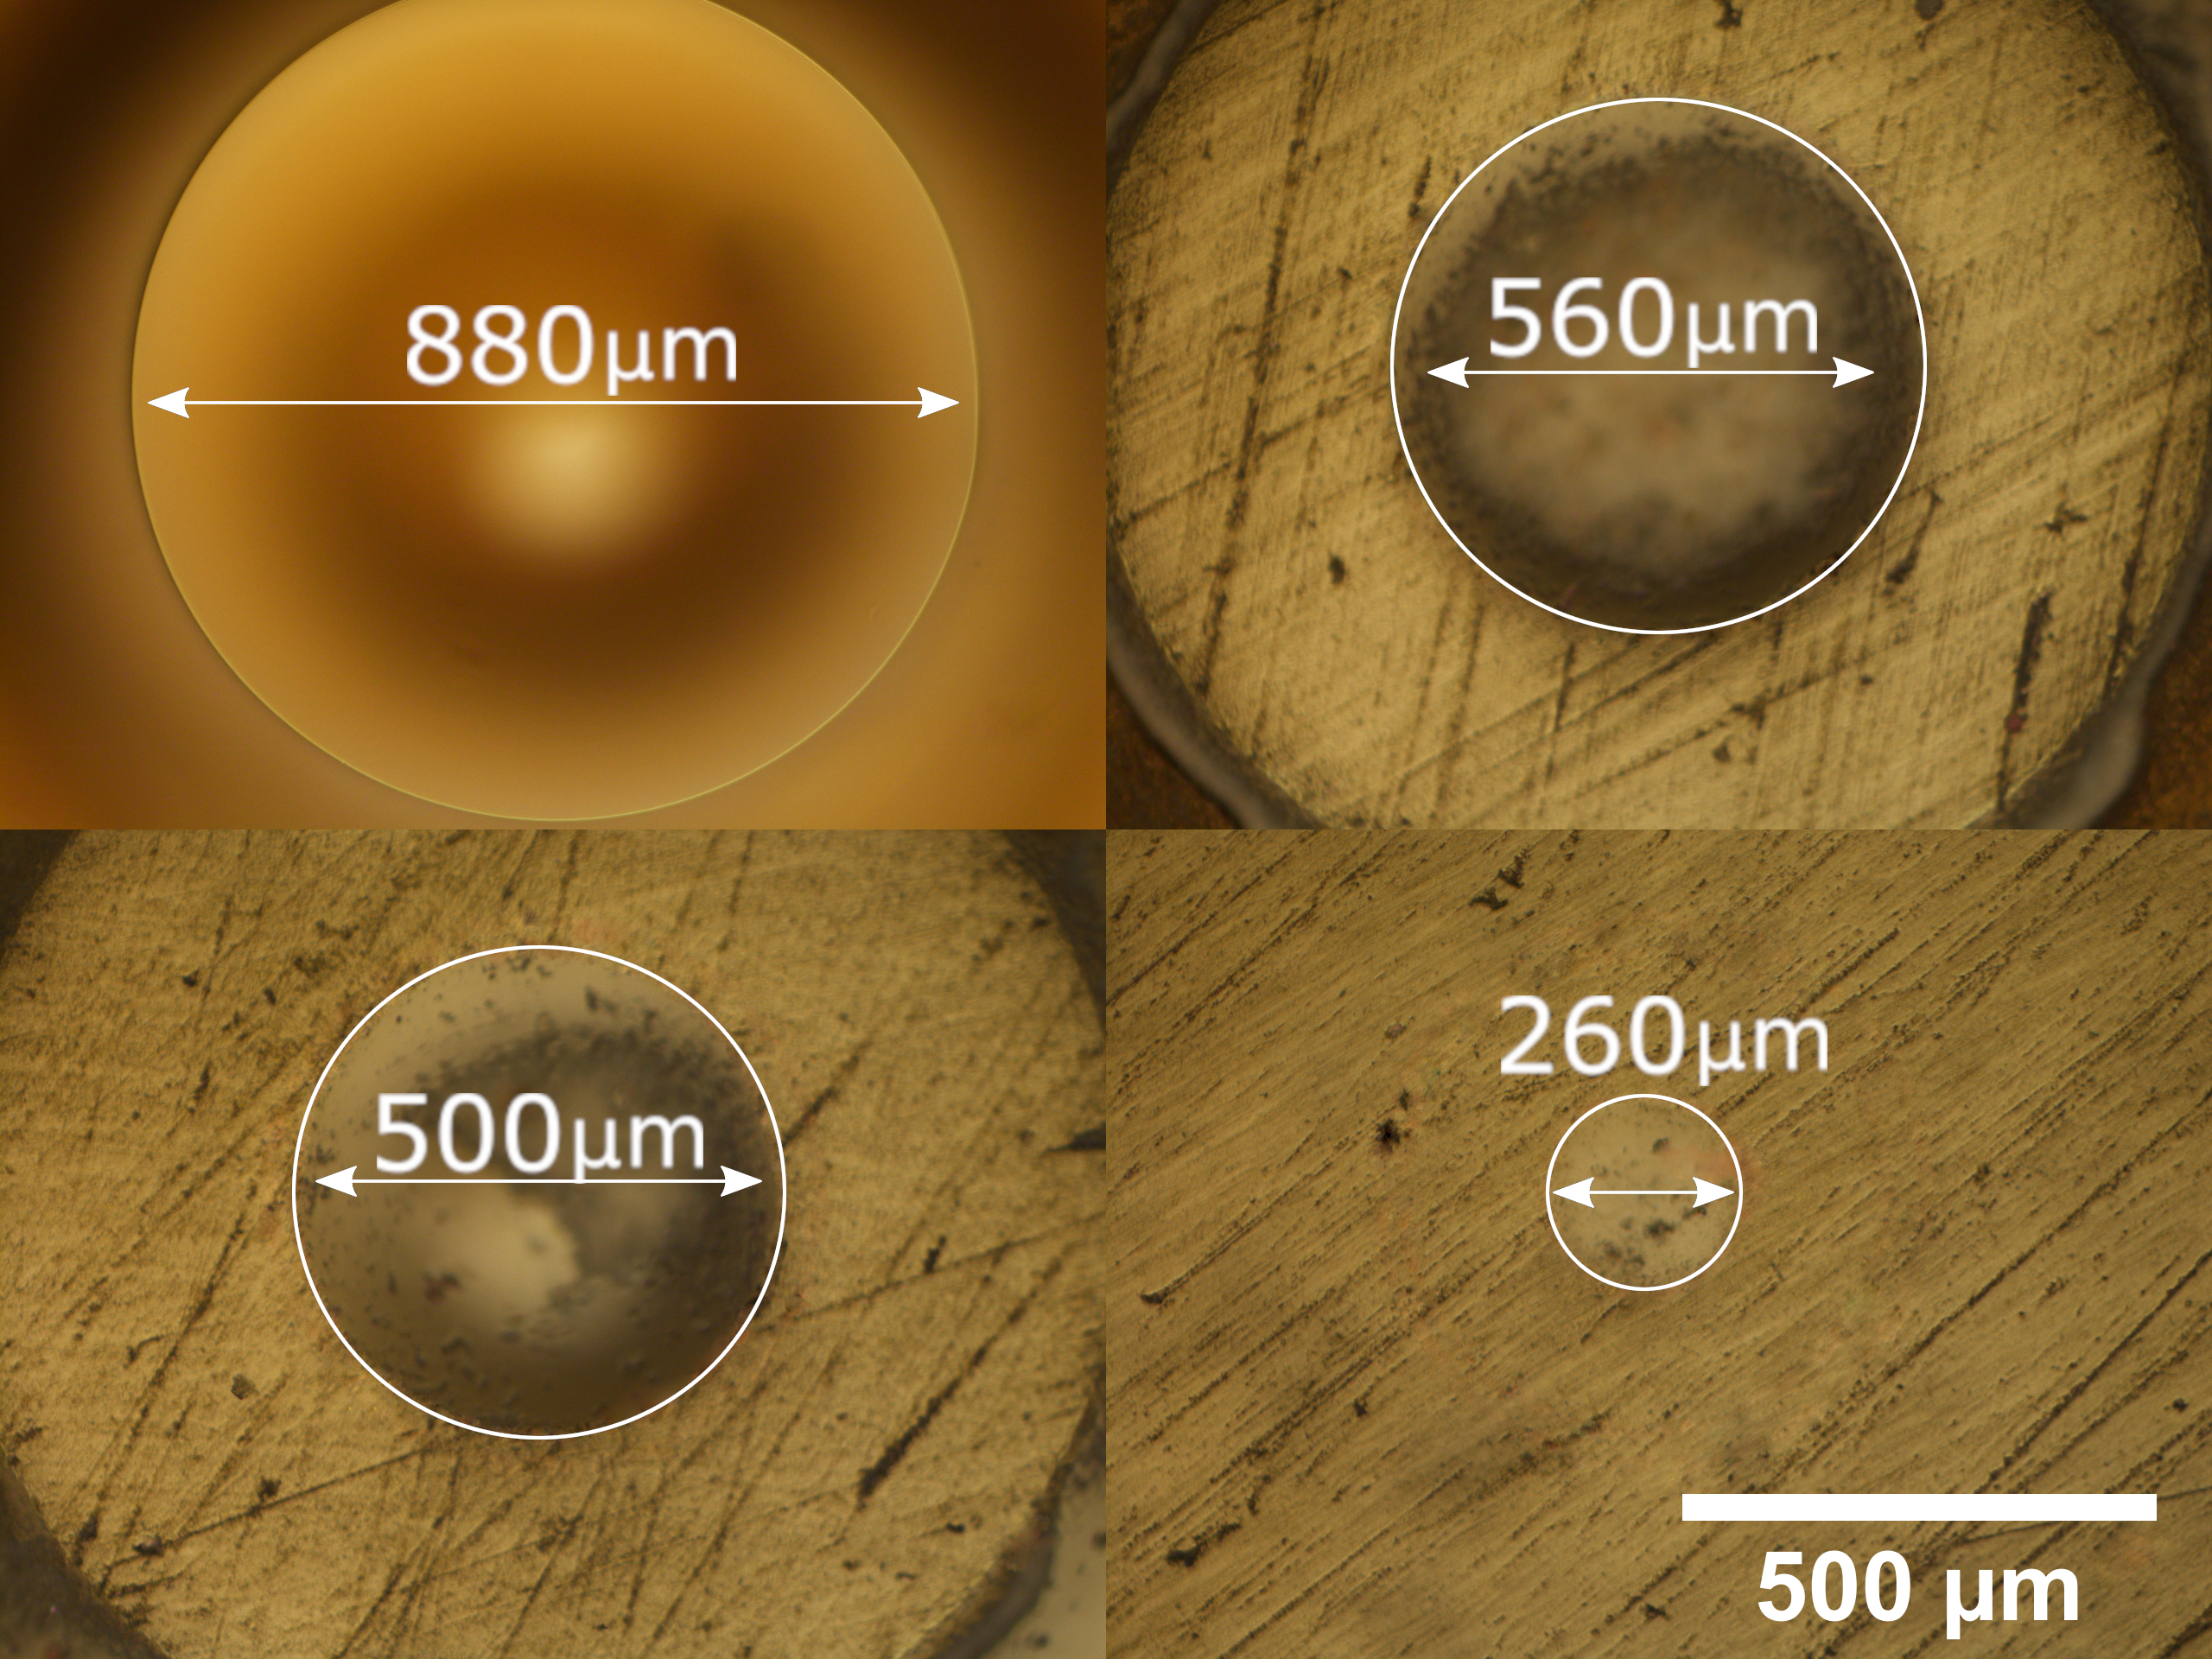
\includegraphics[scale=0.5]{source/grinding/grinding}
	\caption{The microscope images show how the mirror diameter gets smaller during the grinding procedure. The protective layer can be seen over the entire sample in the top left and in the center region in the other images. The sandpaper leaves clearly visible marks wherever it removes material. (Images were digitally enhanced, microscope indicators were removed)}
	\label{fig:GrindingMicroscope}
\end{figure}
Getting the mirrors to a diameter $D=200\um$ is nearly impossible with this method. This coupled with the high risk of destroying the mirror itself makes this the most difficult step of the fabrication process. More problems and possible improvements will be discussed in \autoref{ChapProblems} and \autoref{ChapSolutions}.

\subsection{Cleaning}
The grinding procedure where the mirrors are dimensioned properly causes a lot of dirt on the mirror and the area around it. Furthermore, the dried optical cleaning liquid which was used as a protection layer is still inside the mirror. To remove the dirt and the protection layer residuals we apply the cleaning liquid again and wait for another six hours. After that, a pincer can be used to carefully peel of the newly dried layer, hopefully removing any dirt and residuals on the mirror. While not as difficult as the grinding procedure, cleaning still bares the risk of ripping the mirror from the rest of the material.

\begin{figure}[H]
	\includegraphics[scale=0.25]{source/cleaning_good_scale}
	\includegraphics[scale=0.25]{source/cleaning_bad_scale}
	\caption{On the \textit{left} side a successfully cleaned mirror can be seen. Regardless of the success, scratch marks are clearly visible along the border of the mirror. On the \textit{right} side a site of a mirror, ripped out while cleaning can be seen.}
\end{figure}
\chapter{Results}
So far we have looked at the theoretical background of cavity feedback cooling and have described in detail how the cavity mirrors have to be made and what requirements they have to meet. The following chapter will present the findings of this work and discuss also which steps have been deemed unstable or unfeasible and how they can be improved.

\section{Stamp fabrication}
One core aspect was the fabrication of the stamps which are meant for imprinting the actual mirror shapes. In \autoref{ChapStampFabrication} we have seen in detail how the process is supposed to be implemented based on the observations made during earlier tests. The measured and the calculated quantities of the fabricated stamps are summarized in \autoref{table:CalcMirrorData}.
\begin{table}[H]
	\begin{tabular}{ccccccc}
	\hline
\textbf{Sample} & \textbf{$\mathbf{R\;[\um]}$} & \textbf{$\mathbf{w_0^*\;[\um]}$} & \textbf{$\mathbf{d_{\si{Beam}}^*\;[\um]}$} & \textbf{$\mathbf{D^*\;[\um]}$} & \textbf{$\mathbf{h^*\;[\um]}$} \\
	\hline
	1.1 & 891 & 14.84 & 44.80 & 136.84 & 2.63 \\
	1.2 & 788 & 13.75 & 45.47 & 141.84 & 3.20 \\
	1.3 & 818 & 14.09 & 45.20 & 140.08 & 3.00 \\
	1.4 & 750 & 13.28 & 45.95 & 144.65 & 3.49 \\
	1.5 & 744 & 13.20 & 46.05 & 145.16 & 3.55 \\
	1.6 & 898 & 14.91 & 44.77 & 136.58 & 2.60 \\
	1.7 & 719 & 12.83 & 46.52 & 147.62 & 3.80 \\
	1.8 & 884 & 14.78 & 44.82 & 137.08 & 2.66 \\
	1.9 & 769 & 13.52 & 45.69 & 143.18 & 3.34 \\
	1.10 & 709 & 12.69 & 46.73 & 148.70 & 3.91 \\
	1.11 & 734 & 13.06 & 46.22 & 146.08 & 3.64 \\
	2.1 & 797 & 13.86 & 45.38 & 141.29 & 3.14 \\
	2.2 & 790 & 13.77 & 45.46 & 141.76 & 3.19 \\
	2.3 & 857 & 14.50 & 44.95 & 138.20 & 2.79 \\
	2.4 & 783 & 13.69 & 45.53 & 142.21 & 3.24 \\
	3.1 & 813 & 14.04 & 45.24 & 140.33 & 3.03 \\
	\hline
\end{tabular}
	\caption{The table shows the measured stamp radii $R$ alongside the calculated (*) values for the expected beam waist $w_0$, the beam diameter on the mirror surface $d_{\si{Beam}}$, the diameter of the mirror $D$ and the depth of the mirror $h$. Based on the resolution of the images, the radii can be considered accurate up to $\pm 5\um$.}
	\label{table:CalcMirrorData}
\end{table}
The mean radius across the fabricated stamps is $797\um$ with a standard deviation of $59\um$. This is actually a quite good result because the standard deviation always keeps the radii confined to a range which works for our purposes. As discussed in \autoref{ChapMeasurement}, when $R$ of the stamps, which should coincide with the radius of curvature, and the cavity length $L$ are fixed, the beam waist $w_0$ will change to fit, which is a property of the Gaussian mode populating the cavity. The high reliability and the accurate estimation of the mirror dimensions from the fabricated stamps is one important steps towards the successful fabrication of the cavity mirrors.

\section{Material properties}\label{ChapMatProp}
Until now we have not talked a lot about the materials involved in this fabrication process. Namely these are SiO2 (glass) and a polymer called OrmoComp (Manufacturer: Microresist). The glass serves as the material for the stamps and the polymer is the medium in which the mirrors are imprinted. Going into this project we did not know whether these materials would succeed in producing the required surface roughness or not.\\
To asses the surface roughness of both materials we used an AFM (Atomic force microscope) to measure the RMS (root-mean-square) height deviation or roughness of the surface. The measurements of the stamps were conducted over multiple locations to see how they agree with each other. The result for the stamps was a \textit{mean} RMS of $0.315\nm$ with a \textit{standard deviation} of $0.051\nm$ (forward and backward measurements have been included in this calculation). A special fixture had to be made in order to measure the stamps under the AFM.\\
\begin{figure}[H]
	\includegraphics[scale=0.5]{source/stamp_rms}
	\caption{A ten by ten micrometer AFM scan of the surface near the tip of the glass stamp. Measurements taken at different locations yielded similar looking results.}
\end{figure}
Multiple measurements also were conducted on a flat portion of cured but not stamped OrmoComp polymer. To produce this sample the steps described in \autoref{ChapCoverslipPreparation} were followed. The result for the polymer was a \textit{mean} RMS of $0.326\nm$ with a \textit{standard deviation} of $0.01\nm$ (forward and backward measurements have been included in this calculation). The roughness of the stamp and the polymer are therefore very similar.\\
From these measurements we were able to conclude that the material properties of the stamps and the polymer used as imprinting medium both meet the specifications ($\si{RMS}<0.6\nm$). 

\begin{figure}[H]
	\includegraphics[scale=0.5]{source/OrmoComp_rms}
	\caption{A ten by ten micrometer AFM scan of the OrmoComp surface. Without any imprinting it can be seen that the surface of the polymer is very smooth. Other measurements yielded a similar picture.}
\end{figure}

\section{Mirror fabrication}\label{ChapMirrorFab}
Previously, we looked at the requirements that the materials involved in the process have to fulfil and how good the stamps are that we use for the mirror fabrication. Now we turn our attention at the mirrors that were actually fabricated while using this process. In \autoref{ChapGrinding} we have seen that the mirrors are ill-dimensioned, making the grinding step necessary. In this section we will look at various methods that were used to do the imprinting. These different methods were used to rule out imprecise control of the stamp as the cause of the ill-dimensioned mirrors.

\subsection{Tip station imprinting}
The first method used for imprinting involved a tip station consisting of an optical microscope and a baseplate with a micrometer screw and a pedestal to put the coverslip with the polymer layer onto. To see how close the stamp is to the polymer surface a tilted mirror was used to look sideways onto the sample (see \autoref{fig:TipStation}). To do the imprinting the procedure is to lower the stamp as close as possible to the surface until contact is made but without going into the material. From \autoref{table:CalcMirrorData} we know how deep the mirror has to be in order to match the diameter we aim for. This depth is then achieved by turning the screw accordingly. After that a UV light (US460 Lightpen) is used to cure the still fluid polymer.\\
None of the mirrors produced using this method had the required diameter of $200\um$ but rather a diameter of about $800\um$.  At the beginning it was unclear wherein the problem lies. One assumption was that the micrometer screw together with visual feedback are not precise enough for imprinting the mirrors. As it turned out this was not in fact the case. However, for this reason an alternative approach was tested. In the end, the polymer creeping up the stamp during imprinting was identified as the cause of the problem.

\begin{figure}[H]
	\includegraphics[scale=1]{source/tip_station_compressed}
	\caption{The micrometer screw controls the height of the glass stamp. With the microscope that is directed at the tilted mirror next to the pedestal, the distance of the stamp to the polymer can be seen.}
	\label{fig:TipStation}
\end{figure}

\begin{figure}[H]
	\includegraphics[scale=0.6]{source/mirror_too_large}
	\caption{All mirrors fabricated ended up having a diameter which was too large (approximately $800\um$, the aim was $200\um$). As it turned out this was due to the polymer creeping up the glass stamp during imprinting.}
\end{figure}

\subsection{Inverted microscope imprinting}
The suspicion that the microscope looking sideways onto the polymer surface is an insufficient tool to control the imprinting depth of the stamp into the polymer led to a different approach. In this approach the sample is placed over a microscope which then is focused to the surface. To estimate how far away the stamp is, the focus is adjusted to the tip of the stamp.

\begin{figure}[H]
	\includesvg[scale=0.65]{source/inverted_microscope}
	\caption{This method uses an upside-down microscope mounted below the sample to estimate the distance of the stamp to the polymer surface. Moving the setup up and down allows focusing on different objects. With the objective used, a resolution on the nanometer-scale is possible.}
\end{figure}
In our lab environment this setup required a lot of preparation and took a lot of time to implement. Thanks to the objective which was used for the focusing, a resolution on the nanometer-scale is possible. Nevertheless, after completing the imprinting with this method the diameter was still too large. However, through the microscope it was clearly visible that the polymer was in fact creeping up the glass stamp, therefore lending evidence to the conclusion that the problem is not the control of the stamp.

\subsection{Grinding and results}
The fact that all imprinted mirrors were too deep and had a diameter too large for the utilization in a microcavity means that sandpaper had to be used to dimension the mirrors properly. The consequence of using this sandpaper method is that it requires a lot of attention not to remove too much material. \autoref{table:MirrorRMSResults} shows the RMS values extracted from the mirrors where grinding and subsequent cleaning was successful.\\
In the end we were only able to produce four mirrors that did not break during the last two processing steps. In summary it can be said that the mean RMS over the mirrors is $\si{RMS}=1.9\nm$ and if we remove measurement artifacts and grains by software we have $\si{RMS}=1.7\nm$. These results show that the mirrors do not meet the surface roughness requirement of $\si{RMS}<0.6\nm$. This means that they would lead to losses of around $100$ to $200\ppm$ if used in a cavity.

\begin{table}[H]
	\begin{tabular}{cccc}
	\hline
	\textbf{RMS $[\nm]$} & \textbf{Error $[\nm]$} & \textbf{RMS* $[\nm]$} & \textbf{Error* $[\nm]$} \\
	\hline
	1.96 & 0.43 & 1.81 & 0.43 \\
	1.70 & 0.04 & 1.35 & 0.03 \\
	1.87 & 0.02 & 1.70 & 0.01 \\
	2.09 & 0.03 & 1.93 & 0.02 \\
	\hline
	\end{tabular}
	\caption{The table shows the RMS values of the mirrors where grinding and cleaning was successful. The first column shows the average value of the forward and backward AFM scans. The second column shows the difference of the forward and backward scan which is considered the measurement error. The last two columns, marked with (*), show the results if grains and measurement artifacts are removed with post processing software (Gwyddion 2.52). The first measurement also seems to be less trustworthy than the other samples.}
	\label{table:MirrorRMSResults}
\end{table}


\begin{figure}[H]
	\includegraphics[scale=1]{source/grinded_cleaned_compressed}
	\caption{A cavity mirror after grinding and cleaning. It can be seen that the outer ring of the mirror has some scratches in it. The scratches were probably caused by the rough sandpaper ($30\um$).}
\end{figure}

\section{Challanges}\label{ChapProblems}
During the entirety of this chapter we have looked at the results of all the different fabrication processes that make up the content of this project. While we were able to implement stable processes for the stamp fabrication, silanization and automated measurements procedures, other goals were not reached. Most importantly it was not possible during the course of this project to produce mirrors with a smooth enough surface to send them in for coating.\\
To analyze this problem, measurements of the different materials were taken and the glass stamps as well as the OrmoComp polymer were ruled out as direct causes of the roughness problem. A more likely source of the problem are the last steps of the process: Grinding and cleaning. Especially grinding cannot be controlled very well and has caused a lot of mirrors to break during fabrication. Since the depth of the mirrors was estimated to be around $3\um$ which is also the roughness of the smoothest sandpaper used while grinding, we see that there is not much room for error. The cleaning process also bares a high risk. If the optical cleaning liquid is not removed carefully, the entire mirror can be ripped off or be damaged otherwise. Those arguments are strong indicators that the last two steps are the cause for the roughness problem but there is no conclusive evidence yet and further tests will be necessary.

\section{Possible solutions/improvements}\label{ChapSolutions}
In the last section we have identified the grinding and cleaning steps as the likely cause for the surface roughness which is too high in the fabricated mirrors. The most obvious improvement would be to just omit both processing steps altogether. We have to understand why the mirrors get too wide and therefore too deep. As discussed in \autoref{ChapMirrorFab}, the control of the stamp during imprinting was ruled out as the problem. Another source of the problem could be the silanization process as it may not work as intended. After calling Microresist, the manufacturer of OrmoComp we found out that the creeping is an intended effect of the polymer and ensures that every detail of the stamp is captured properly. According to Microresist this has nothing to do with silanization.
With this knowledge it was possible to develop a new idea for the imprinting process. Since the way OrmoComp is supposed to be used is with arrays of stamps where a "ceiling" limits the height the polymer can lift itself up we also need a ceiling or walls in our method (see \autoref{fig:newIdea}).

\begin{figure}[H]
	\includesvg[scale=0.45]{source/new_stamp_idea}
	\caption{Since OrmoComp tries to capture every detail by creeping up the stamp the solution to prohibit this behaviour is to add walls which retain the polymer. By adding the glass coverslip to the stamp with a hole that has exactly the diameter which is needed for the mirror ($200\um$) the mirror wont get too large and neither too deep.}
	\label{fig:newIdea}
\end{figure}

To only get the mirror without the excess material shown in \autoref{fig:newIdea}, a spin coater can be used. After the polymer has been put into the mould it can be cured. The question remains if the mirror will stay inside of the coverslip if the stamp is removed or if it comes out with the stamp. In both cases the retrieval of the mirror should be possible without much difficulties.\\
The challenge of this method is how to get a hole with the correct diameter into the coverslip. One method could be to use ultra-short laser pulse ablation to create the hole.  Unfortunately, due to the lack of equipment and time constraints we were not able to test this method. As a first step, tests were conducted with steel plates and holes with $1\mm$ diameter. These tests showed that the OrmoComp can successfully be restricted in its expansion.
\chapter{Summary and Outlook}
The goal of this work was to develop and evaluate a method to fabricate spherical microcavity mirrors. The purpose of theses mirrors is their utilization as part of a microcavity for the use in a trapping experiment. The small mode volume of the microcavity would allow a high sensitivity enabling the position measurement of a levitated nanosphere.

The process was developed and the various steps have been tested and evaluated. The melting of standard communication glass fibers into spherical glass stamps was achieved with the construction of a rotating fixture and the utilization of a small blow torch for melting. The resulting stamps were measured to determine the ROC which has to be between $0.7\mm$ and $1.0\mm$. All produced stamps had the proper dimensions. Furthermore, the stamps were measured with the AFM to determine their surface roughness since the RMS value is a key quantity in assessing losses of the final mirrors. AFM measurements showed that the glass stamps as well as the OrmoComp polymer used to imprint the mirrors into have $\si{RMS}<0.4\nm$ which meets the requirement which was set to be an RMS smaller than $0.6\nm$.

To preserve the good surface quality of both stamp and polymer during imprinting a silanization treatment was evaluated and tested to add an anti-adhesive layer to the stamp. Tests without the application of this layer resulted in the stamps ripping apart when trying to remove them from the cured mirrors.

When using the stamps to imprint the mirrors into the polymer a problem was discovered that proved to be difficult to be localized. The mirrors produced were always too wide and too deep, which rendered them unusable for the trapping experiment. Tests with different imprinting methods finally led to the conclusion that the problem was in fact the polymer creeping up the glass stamps during imprinting. This behavior was also confirmed by the manufacturer of the polymer. 

Grinding the mirrors with sandpaper has been shown to be a possible solution to get the mirrors to the proper dimensions. However, grinding was deemed to be very hard to control and greatly reduced the yield of produced mirrors. Of the four successfully produced mirrors all had $\si{RMS}\approx 1.7\nm$ which is about three times higher than required. Identifying the grinding procedure as the likely cause of this problem led to the conclusion that omitting this step altogether would be an important obstacle to overcome.

To overcome this obstacle a new method for imprinting was developed which uses additional glass structures to contain the polymer in the volume required. The fabrication of this new stamp was partly tested but due to time constraints the real evaluation will be the goal of a future project.
\appendix
\chapter{Appendix}
\section{extract\_ROC.py}
\UseRawInputEncoding
\begin{lstlisting}
"""
File:           extract_ROC.py
Author:         Dominik Werner, 2018
Description:    This script opens images taken on the microscope of the fabricated stamps and tries to extract the ROC
"""

import numpy as np
import matplotlib.pyplot as plt
from PIL import Image
from skimage import measure
from scipy.optimize import curve_fit
from skimage import feature, color
import os

# import settings
date = '05.12.2018'
sample = 'tip4'

show_single_image = False   # if set to true only opens one image and displays the data (else process entire folder)
summary_file = 'radii.csv'  # file to save ROC data to for further processing

required_surface_diameter = 0.3  # mm, used for identifying ROC extraction contour

scale = 520.0010    # px/mm, metric


def find_sample(image):
    '''
    Locate the sample with the molten glas droplet in the image.
    :param image: image
    :return: contour that is most likely the droplet as well as the center of the contour and its width and height.
    '''
    contours = measure.find_contours(image[..., 0], 115)    # search contours
    radius = 0
    for c in contours:  # loop through all the contours to find the largest -> most likely to be the droplet
        dev_h, dev_w = np.std(c, axis=0)    # standard deviation determines the extent of the droplet
        r = np.sqrt(dev_w**2 + dev_h**2)    # calculate the radius of the found contour
        if r > radius:  # if the radius is bigger than the largest up to this point select this candidate
            radius = r
            contour = c
            width = dev_w * 2
            height = dev_h * 2
    y0, x0 = np.mean(contour, axis=0)
    return contour, x0, y0, width, height


def find_circle(image):
    '''
    Use canny edge detection and the ransac algorithm to detect a circle in a given image.
    :param image: image containing the circle
    :return: center point coordinates x and y as well as the radius
    '''
    edges = feature.canny(color.rgb2gray(image), sigma=2)
    '''plt.figure()
    plt.imshow(edges)
    plt.show()'''
    points = np.array(np.nonzero(edges)).T
    model_robust, _ = measure.ransac(points, measure.CircleModel, min_samples=3, residual_threshold=2, max_trials=1000)
    cy, cx, r = model_robust.params
    return cx, cy, r


def circle(x0, y0, r):
    '''
    Outputs a collections of x and y coordinates for plotting a circle.
    :param x0: center point x coordinate
    :param y0: center point y coordinate
    :param r: radius
    :return: x, y collections
    '''
    phi = np.linspace(0, 2*np.pi)
    x = x0 + r * np.cos(phi)
    y = y0 + r * np.sin(phi)
    return x, y


def do_sphere_analysis(path):
    print('opening image...')
    im = np.array(Image.open(path))     # load selected image

    # find sample in the image (the largest contour that can be found)
    print('searching for sample in image...')
    contour, x0, y0, width, height = find_sample(im)

    # define region of interest
    expansion_factor = 1.5

    x_min = x0 - width / 2 * expansion_factor
    x_max = x0 + width / 2 * expansion_factor
    y_min = y0 - height / 2 * expansion_factor
    y_max = y0 + height / 2 * expansion_factor

    # make sure that the indices for the region of interest are bounded
    print('determining region of interest...')
    image_height, image_width, _ = im.shape
    if x_min < 0: x_min = 0
    if y_min < 0: y_min = 0
    if x_max > image_width - 1: x_max = image_width - 1
    if y_max > image_height - 1: y_max = image_height - 1

    # extract region of interest from image for circle detection
    image_roi = im[int(y_min):int(y_max), int(x_min):int(x_max)]

    # extract the contour that lies within the region of interest
    print('extracting contour...')
    mask = (contour[:, 1] > x_min) & (contour[:, 1] < x_max) & (contour[:, 0] > y_min) & (contour[:, 0] < y_max)
    contour_x = contour[mask, 1]
    contour_y = contour[mask, 0]

    # find the angle in which the sample is oriented
    print('estimating droplet center...')
    roi_intersection1 = np.asarray([contour_x[0], contour_y[0]])
    roi_intersection2 = np.asarray([contour_x[-1], contour_y[-1]])
    diff_vec = roi_intersection2 - roi_intersection1
    sample_orientation = np.arctan2(diff_vec[1], diff_vec[0]) + np.pi / 2   # +90° because the orientation is perpendicular
    print('The sample seems to be oriented at an angle of {}°.'.format(round(sample_orientation * 180 / np.pi), 2))

    # rotate (around roi center) the contour such that the maximum of the x part can be used to estimate the center of the droplet
    contour_x_rotated = np.cos(-sample_orientation) * (contour_x - x0) - np.sin(-sample_orientation) * (contour_y - y0) + x0
    contour_y_rotated = np.sin(-sample_orientation) * (contour_x - x0) + np.cos(-sample_orientation) * (contour_y - y0) + y0

    # find cap of the droplet for the circle fit -> around 300µm of surface diameter are needed in the end
    droplet_center_index = np.argmax(contour_x_rotated)     # get contour index of estimated droplet center
    droplet_center_x = contour_x[droplet_center_index]      # get droplet center x coordinate
    droplet_center_y = contour_y[droplet_center_index]      # get droplet center y coordinate

    safety_factor = 2     # expand the fitting area or shrink it if necessary
    diameter = required_surface_diameter * safety_factor    # required surface diameter of the droplet
    threshold_pixel_count = 4   # additional pixels around the circle fit region of interest to make sure nothing is cut off

    contour_start_index = int(droplet_center_index - diameter / 2 * scale)  # fit contour start index
    contour_end_index = int(droplet_center_index + diameter / 2 * scale)    # fit contour end index
    fit_contour_x = contour_x[contour_start_index:contour_end_index]    # x coordinates of the fit contour
    fit_contour_y = contour_y[contour_start_index:contour_end_index]    # y coordinates of the fit contour
    fit_roi_x_min = np.min(fit_contour_x) - threshold_pixel_count
    fit_roi_x_max = np.max(fit_contour_x) + threshold_pixel_count
    fit_roi_y_min = np.min(fit_contour_y) - threshold_pixel_count
    fit_roi_y_max = np.max(fit_contour_y) + threshold_pixel_count
    roi_fit = im[int(fit_roi_y_min):int(fit_roi_y_max), int(fit_roi_x_min):int(fit_roi_x_max)]  # roi for the circle fit

    #plt.figure()
    #plt.imshow(roi_fit)

    # run circle detection on region of interest (is faster and more accurate than on original image)
    print('fitting circle...')
    cx, cy, radius = find_circle(roi_fit)
    cx += int(fit_roi_x_min)    # translate x coordinate of center point to original image
    cy += int(fit_roi_y_min)    # translate x coordinate of center point to original image
    circle_x, circle_y = circle(cx, cy, radius)   # get coordinates of circle for plotting


    fig = plt.figure()    # create figure
    plt.tight_layout()
    plt.title('radius={} mm'.format(round(radius / scale, 2)))
    ax1 = plt.subplot(1, 1, 1)
    ax1.set_xlim([0, image_width / scale])  # set scaling for x axis -> use mm
    ax1.set_ylim([0, image_height / scale])   # set scaling for y axis -> use mm
    ax1.set_xlabel('x [mm]')
    ax1.set_ylabel('y [mm]')
    ax2 = ax1.twinx().twiny()  # instantiate a second axes
    ax2.imshow(im)  # display image

    # draw the region of interest
    ax2.add_patch(plt.Rectangle((x_min, y_min), width*expansion_factor, height*expansion_factor, fill=False, edgecolor='g'))

    ax2.plot(contour_x, contour_y, color='r')   # draw detected contour
    #ax2.plot(contour_x_rotated, contour_y_rotated, color='b')   # draw detected contour (rotated)
    ax2.plot(circle_x, circle_y)    # draw detected circle
    ax2.plot([droplet_center_x], [droplet_center_y], marker='o')    # draw estimated center of droplet
    ax2.plot(fit_contour_x, fit_contour_y, color='y')

    return fig, radius / scale * 1e3     # return radius in µm


if show_single_image:
    do_sphere_analysis('Samples/{}/{}.TIF'.format(date, sample))
    plt.show()
else:
    csv = open('Samples/{}/Results/{}'.format(date, summary_file), 'w+')
    csv.write('Sample;Radius [µm]\n')

    for file in os.listdir('Samples/{}'.format(date)):
        if not os.path.isdir('Samples/{}/{}'.format(date, file)):
            print('Analyzing image: {} ...'.format(file))
            fig, r_um = do_sphere_analysis('Samples/{}/{}'.format(date, file))
            fig.savefig('Samples/{}/Results/{}.png'.format(date, file))
            csv.write('{};{}\n'.format(file.lower().replace('.tif', '').replace('.png', ''), r_um))

    csv.close()
\end{lstlisting}

\section{extract\_mirror\_dimensions.py}
\begin{lstlisting}
"""
File:           extract_mirror_dimensions.py
Author:         Dominik Werner, 2018
Description:    This script opens calculates the mirror dimensions from measured radii of fabricated stamps
"""

import numpy as np

# input and output files
input_file_path = 'Samples/05.12.2018/Results/radii.csv'
result_file_path = 'Samples/05.12.2018/Results/calculated_mirrors.csv'

# Definitions
desired_cavity_length = 500e-6  # 0.5 mm
cover_slip_thickness = 160e-6  # https://de.vwr.com/store/product/3006241/deckglaeser-menzel-glaeser
ormocomp_layer_thickness = 25e-6  # rough estimate
diameter_factor = 5

pi = np.pi
wl = 1565e-9    # wavelength

focus_waist_from_r_L = lambda R, L: np.sqrt(wl/pi)*(L*(R-L))**(1/4)


def extract_mirror(ROC, name):
    '''
    Extract mirror dimensions from a given ROC
    :param ROC: radius of curvature in m
    :param name: name of the sample
    :return: beam waist at the focus point, beam waist radius at mirror position,
    Gaussian beam diameter on mirror, mirror diameter, mirror depth
    '''
    w0 = focus_waist_from_r_L(ROC, desired_cavity_length)  # beam waist at focus
    k = 2*pi/wl     # wave vector
    zR = pi*w0**2/wl    # Rayleigh range
    n = 1   # refractive index
    th = wl/(pi*n*w0)   # divergence angle
    psi = lambda z: np.arctan(np.divide(z, zR))    # Gouy phase
    R = lambda z: z*(1 + np.power(np.divide(zR, z), 2))     # wave front radius
    z_from_R = lambda R: (R+np.sqrt(R**2-4*zR**2))/2
    w = lambda z: w0*np.sqrt(1 + np.power(np.divide(z, zR), 2))     # beam width

    r1 = ROC  # 1mm
    z1 = z_from_R(r1)
    D = w(z1 + ormocomp_layer_thickness + cover_slip_thickness) * diameter_factor
    D0 = 2*r1*np.arctan(w(desired_cavity_length)/r1)  # Mirror diameter hit by gaussian beam
    h1 = r1 - np.sqrt(r1**2 - D**2/4)  # height of desired mirror

    print('Mirror:', name)
    print('Wavefront Radius: R1 =', r1*1e6, 'µm')
    print('Desired hemispherical cavity length: L =', desired_cavity_length*1e6, 'µm')
    print('Required focal radius: w0 =', w0*1e6, 'µm')
    print('Mirror-Center Distance: d1 =', z1*1e6, 'µm')
    print('Mirror diameter hit by gaussian beam: D0 =', D0*1e6, 'µm')
    print('Desired mirror diameter (opening circle): D =', D*1e6, 'µm')
    print('Height/Depth of desired mirror: h1 =', h1*1e6, 'µm')
    print('Focus width (diameter): w0 =', 2*w0*1e6, 'µm')
    print('Cavity length (hemispherical): L = ', z1*1e6, 'µm')
    print('***************************************************************************************')

    return w0, z1, D0, D, h1


input_file = open(input_file_path, 'r')
result_file = open(result_file_path, 'w+')

result_file.write('Sample;Radius [µm];Cavity Length [µm];Required w0 [µm];'
                  'Beam Diameter on mirror [µm];Mirror Diameter [µm];Mirror Depth [µm]\n')

lines = input_file.readlines()  # read lines with the radii of the measured stamps
for i in range(1, len(lines)):   # skip first line
    line = lines[i]
    cells = line.split(';')
    if len(cells) == 2:
        name = cells[0]
        R = float(cells[1])*1e-6
        w0, L, D0, D, h1 = extract_mirror(R, name)
        result_file.write('{};{};{};{};{};{};{}\n'.format(name, R*1e6, L*1e6, w0*1e6, D0*1e6, D*1e6, h1*1e6))

result_file.close()
input_file.close()
\end{lstlisting}




\backmatter
\bibliographystyle{rene}
%\bibliographystyle{ieeetr}
\bibliography{master_bib}

\cleardoublepage
\thispagestyle{empty}
\section*{Aknowledgements}
I would like to thank Prof. Dr. Lukas Novotny, Dominik Windey and Dr. Ren\'{e} Reimann for the opportunity of working on this semester thesis.

During the entire project I could always rely on the supervision of either Dominik Windey or Dr. Ren\'{e} Reimann if questions of any sort arose. Their knowledge and the time they took to explain the principles of cavity dynamics in the context of this thesis was very much appreciated. Furthermore, I like to thank them for reading this report and being upfront and honest with their criticism, which helped to greatly improve the quality of this work.

Many thanks go to Anna Kuzmina. Her help was not only appreciated but also crucial to many insights that were gained during the course of this work. The many hours which she spent assisting my project were invaluable. She was always patient and precise while helping me and offered a lot of new ideas during the many discussions we had.

Furthermore, I also want to say a special "thank you" to Dr. Martin Frimmer for the many instances where he made suggestions and the many times he gave valuable tips regarding this work.

Additionally, I want to thank Dr. Achint Jain, who assisted me greatly with the AFM measurements and the evaluation of the data, even though he also had to prepare his PhD defense.

Finally, I want to thank every member of the Photonics Laboratory, for all the interesting discussions, the help and the generally friendly, open and inclusive environment I had the privilege to work in.

\end{document}